\subsection{Three New Graphical Models for Statistical Language Modelling \cite{Mnih2007}}

This paper shows how real-valued distributed representations for words can be learned at the same time as learning a large set of stochastic binary hidden features that are used to predict the distributed representation of the next word from previous distributed representations. One of the proposed models significantly outperforms the best $n$-gram models.

The first model is called the \emph{Factored Restricted Boltzmann Machine Language Model (FRBM)}. Each word is represented using a real-valued feature vector of length $N_f$. Let $R$ be an $N_w \times N_f$ matrix with row $i$ being the feature vector for the $i$-th word. The \emph{joint energy} of a sequence of words $w_1, ..., w_n$ is defined as:
$$E(w_n, h; w_{1:n-1}) = -(\sum_{i=1}^n v_i^T R W_i)h.$$
Here matrix $W_i$ specifies the interaction between the vector of hidden variables and the feature vector.

The joint conditional distribution of the next word and the hidden configuration $h$ is defined in terms of the energy function as:
$$P(w_n, h | w_{1:n-1}) = \frac{1}{Z_c} \exp(-E(w_n,h; w_{1:n-1})),$$
where $Z_c$ is a context-dependent normalization term. The conditional distribution of the next word can be obtained by marginalizing over the hidden variables.
\begin{figure}
  \centering
  % Requires \usepackage{graphicx}
  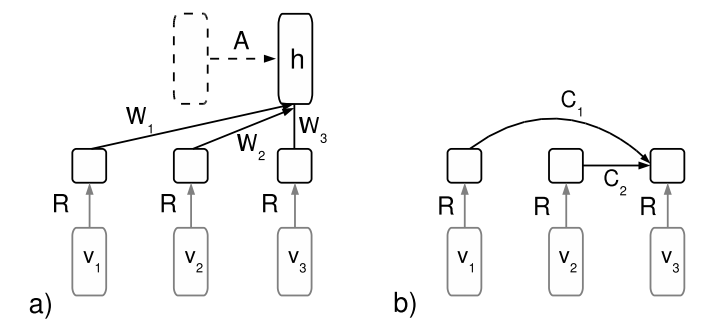
\includegraphics[width=.6\linewidth]{Minh07-RBM.png}\\
  \caption{a) The diagram for FRBM and TFRMB. The dashed part is included only for the TFRBM; b) The diagram for the log-bilinear model.}\label{fig:Minh07-RBM}
\end{figure}

The second model is called the \emph{Temporal Factored RBM (TFRBM)}. The basic idea is to make a simple extension to the factored RBM language model. Suppose we want to predict word $w_{t+n}$ from $w_1, ..., w_{t+n-1}$ for some large $t$. The method applies a separate instance of the model to words $w_\tau, ..., w_{\tau+n-1}$ for each $\tau$ in $\{1, ..., t\}$. In order to propagate context information forward, it further introduces directed connections from $h^\tau$ to $h^{\tau+1}$, and computes the hidden state of model $\tau+1$ using the inputs from the hidden state of model $\tau$ as well as its visible units. Figure \ref{fig:Minh07-RBM} (a) shows the diagram for the temporal FRBM.

The third model is called the \emph{log-bilinear language model}. The energy function of this model is specified as:
$$E(w_n; w_{1:n-1}) = -(\sum_{i=1}^{n-1} v_i^T R C_i)R^T v_n - b_r^T R^T v_n - b^T_v v_n.$$
In the FRBM energy function the interaction is between the word feature vectors and the hidden variables, whereas in this model the interaction is between the feature vectors for the context words and the feature vector for the predicted word. Intuitively, the model predicts a feature vector for the next word by computing a linear function of the context word feature vectors. Then it assigns probabilities to all words in the vocabulary based on the similarity. This model is similar to the energy-based model proposed in \cite{Bengio2003A}. However, the model proposed here uses a bilinear energy function, while the energy function in \cite{Bengio2003A} is a one-hidden-layer neural network. Figure \ref{fig:Minh07-RBM} (b) shows a diagram of the log-bilinear language model.

In the experimental study, the paper evaluates the proposed models using the \emph{Associated Press News (APNews)} dataset consisting of a text stream of about 16 million words. In the first experiment, it is shown that three of the four network models are competitive with $n$-gram models. The best results were obtained by averaging with the temporal network model, resulting in 21\% reduction in perplexity over the best $n$-gram model. In the second experiment, it is also shown that the log-bilinear models clearly outperform the $n$-gram models.
